\documentclass[a4paper,12pt]{scrartcl}
\usepackage[ngerman]{babel}
\usepackage{graphicx} %Bilder einbinden
\usepackage{amsfonts,amsmath,amssymb,amsthm} %erweiterte Mathe-Zeichen
%\usepackage{minted}
\usepackage{mathtools}
\usepackage[utf8]{inputenc} %Umlaute & Co
\usepackage{fancyhdr}
\usepackage{forloop}
\usepackage{ifthen}
\usepackage{courier}
\usepackage{blkarray}
\usepackage{listings}
\usepackage{tikz}
\usepackage{color}
\usepackage{cancel}
\usepackage{enumerate}
\usepackage{multirow,booktabs,bigdelim}
\pagestyle{fancy}
\usepackage{mathtools}
\usepackage{marvosym}
\usepackage[]{algorithm2e}
\usepackage{pgfplots}
\usepackage{listingsutf8}
\definecolor{kommentar}{rgb}{0.75,0.49,0.07}
\newcommand{\latexcode}[1]{\textcolor{kommentar}{#1}}
\usepackage[normalem]{ulem} % [normalem] to set \emph{} to default behaviour (italic instead of underlining)
\usepackage{mdsymbol}
\DeclarePairedDelimiter{\ceil}{\lceil}{\rceil}
\DeclarePairedDelimiter{\floor}{\lfloor}{\rfloor}
\fancyhf{}
\rhead{Informatik II Thorsten Grust}
\lhead{Skript SS15 Finn Ickler}
\newcommand{\linie}{\noindent\makebox[\linewidth]{\rule{\paperwidth}{0.4pt}}}
\newcommand{\auf}{\textless}
\newcommand{\zu}{\textgreater}
\newcommand{\eval}{$\longrightsquigarrow$}
\renewcommand{\i}{\item}
\renewcommand{\t}{\text}
\newcommand{\arge}[1]{\auf $e_{#1}$\zu}
\newcommand{\argt}[1]{\auf $t_{#1}$\zu}
\newcommand{\argcomp}[1]{\auf $\t{comp}_{#1}$\zu}
\newcommand{\argid}[1]{\auf $\t{id}_{#1}$\zu}
\lstset{
  language=Macht der Abstraktion
}
\author{Finn Ickler}
\title{Informatik II Skript Sommersemester 2015}
\begin{document}
\maketitle
\tableofcontents
\newpage
\section{14.4.2015}
\section*{Scheme}
\underline{A}usdr\"ucke , \underline{A}uswertung und \underline{A}bstraktion\\
\subsection*{Dr Racket}
\fbox{
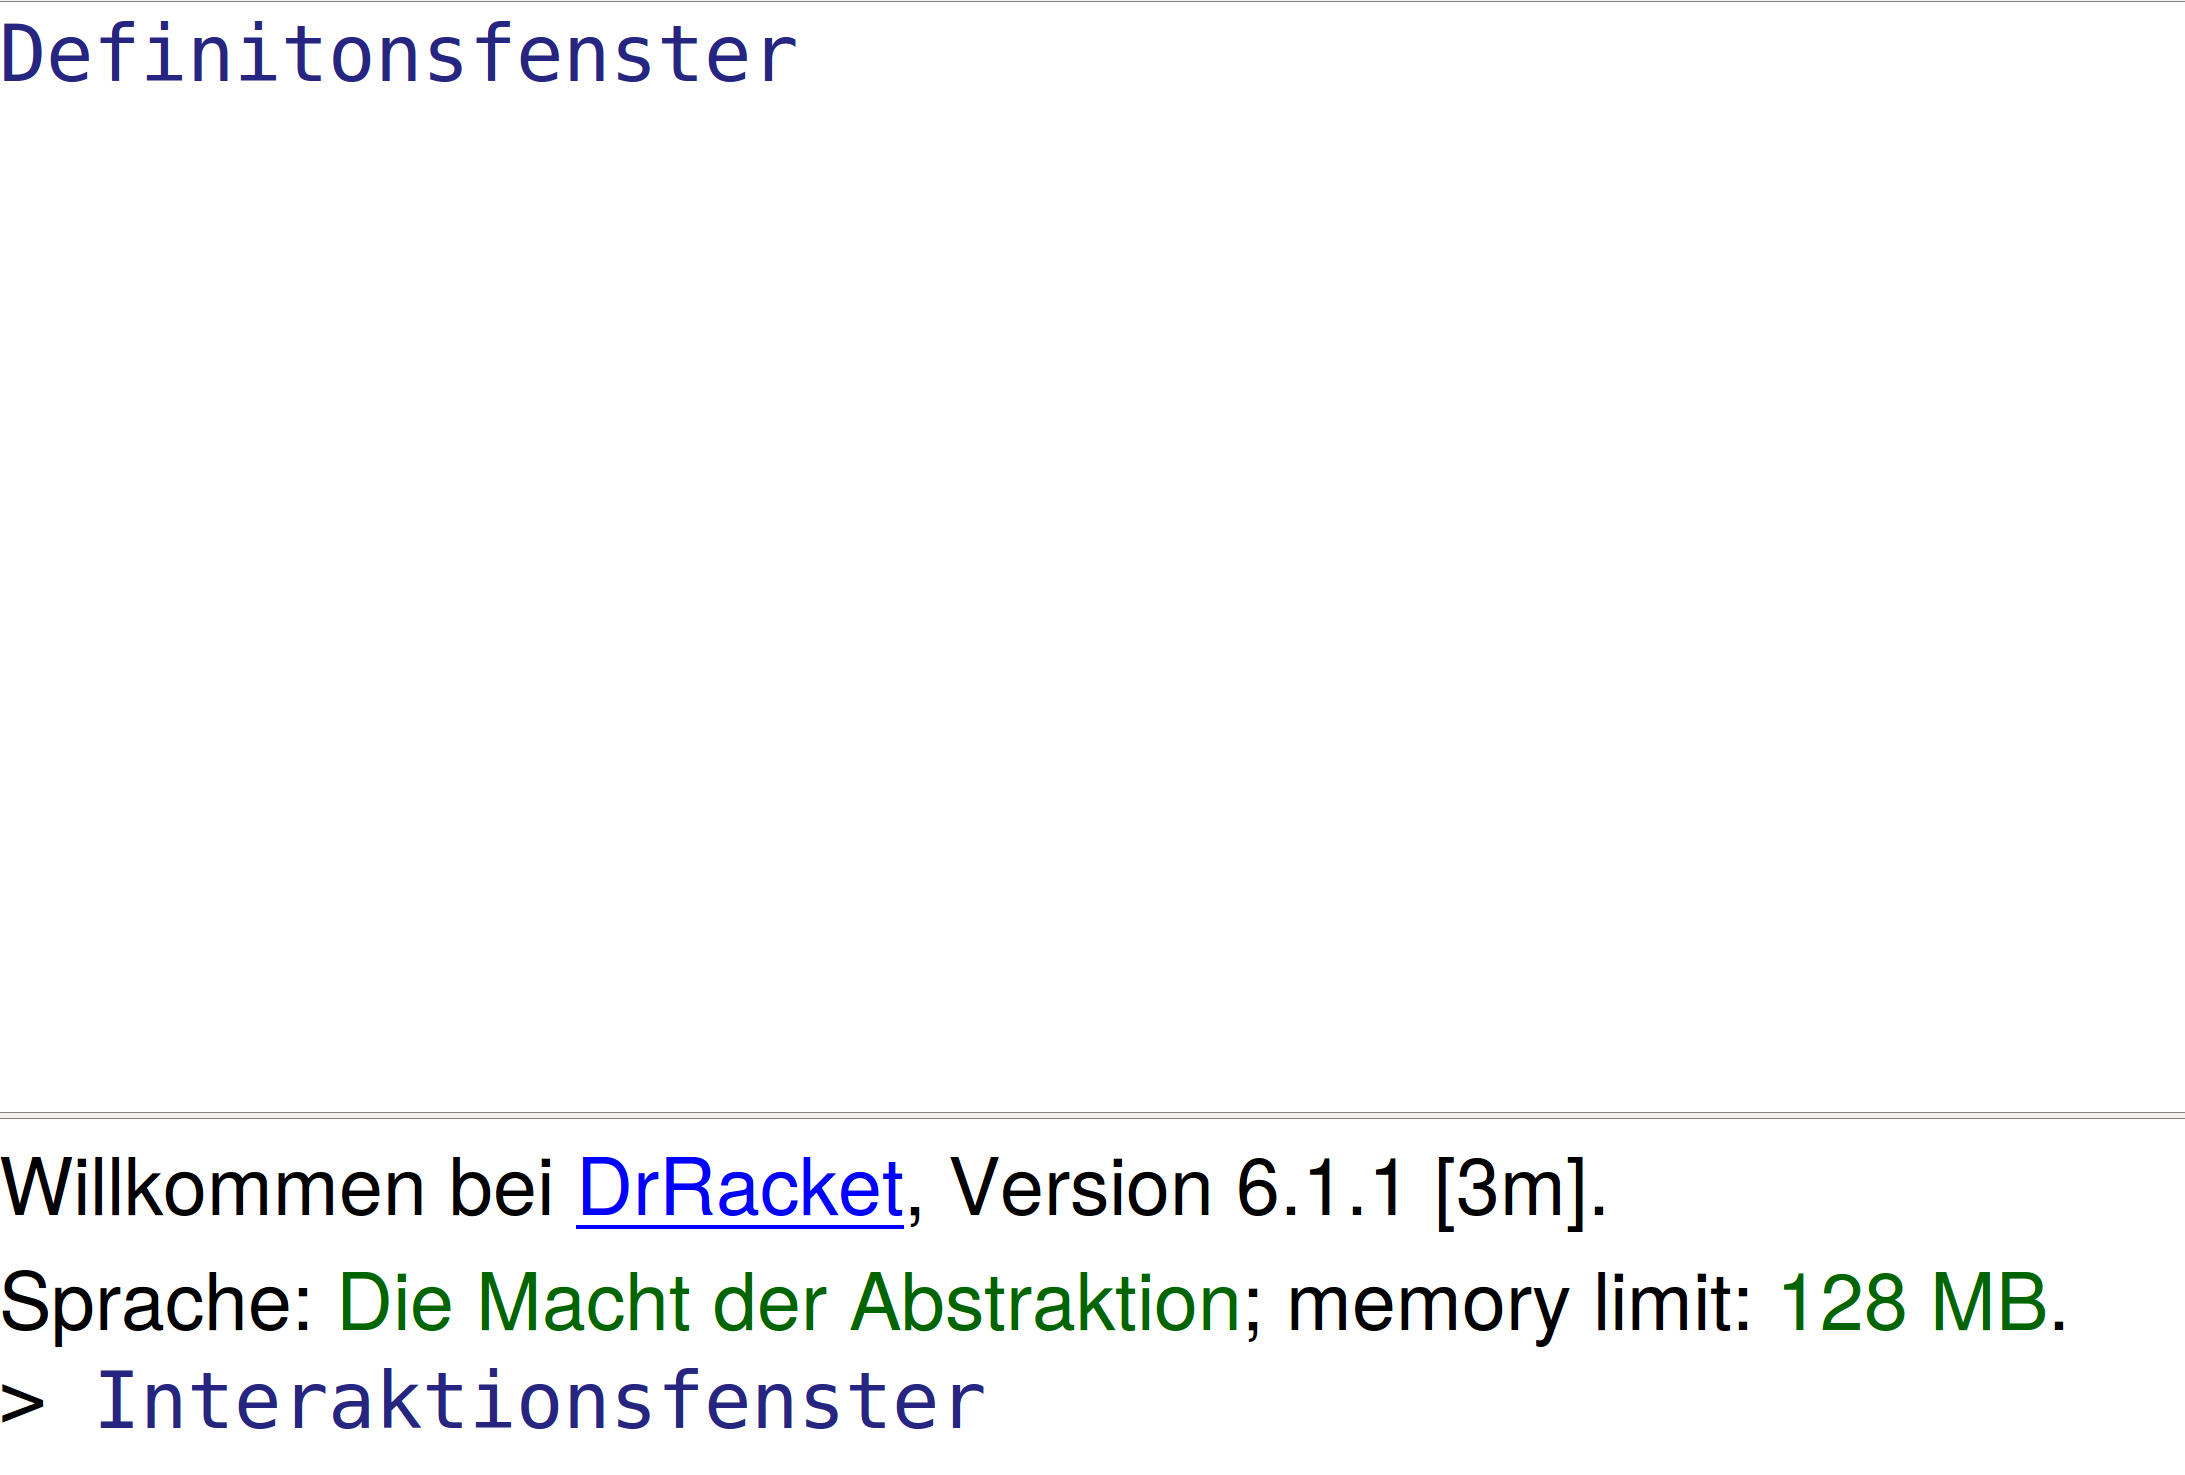
\includegraphics[scale=0.15]{drracket}}\\
Die Anwendung von Funktionen wird in Scheme ausschlie\ss lich in Pr\"afixnotation durchgef\"uhrt
\bigskip\\
\begin{center}
\begin{tabular}{c|c}
Mathematik & Scheme \\
\hline
$44-2$ & $(- $44 2)\\
$f(x,y)$ & (f x y)\\
$\sqrt{81}$ & (sqrt 81)\\
$9^2$ & (expt 92)\\
$3!$ & (! 3)\\
\end{tabular}\\
Allgemein: (\textless funktion\textgreater \textless argument1\textgreater \textless argument2\textgreater \ldots)
\end{center}
(+ 40 2) und (odd? 42) sind Beispiele f\"ur \underline{Ausdr\"ucke}, die bei \underline{Auswertung} einen Wert liefern.\\
(Notation: \eval)\\
(+ 40 2) $\underbrace{\longrightsquigarrow}_{Reduktion}$ 42\\
(odd? 42) \eval \#f
\bigskip\\
Interaktionsfenster:\hspace*{2.5cm} $\underbrace{Read \rightarrow Eval \rightarrow Print \rightarrow Loop}_{REPL}$\\
\bigskip\\
\underline{Literale} sethen f\"ur einen konstanten Wert (auch: \underline{Konstante}) und sind nicht weiter reduzierbar.\\
\begin{center}
\begin{tabular}{ccc}
Literal &  & Sorte,Typ\\
\hline
\#f ,\#t & (true, false, Wahrheitswert) & boolean\\
"x" & (Zeichenketten) & String\\
0 1904 42 $-2$ & (ganze Zahl) & Integer\\
0.42 3.14159 & (Flie\ss kommazahl) & real\\
1\textbackslash 2, 3\textbackslash 4, -1\textbackslash 10 & (rationale Zahlen) & rational\\

\includegraphics[scale=0.2]{Darth_Vader} & (Bilder) & image

\end{tabular}
\end{center}



\section{16.4.2015}

Auswertung \underline{zusammengesetzter Ausdr\"ucke} in mehreren Schritten (Steps), von ``innen nach au\ss en``, bis keine Reduktion mehr m\"oglich ist.\\
\begin{lstlisting}
(+ ( @\uwave{(+ 20 20)}@ (+ 1 1)) @\eval@ (+ 40 @\uwave{(+ 1 1)}@ @\eval@ (+ 40 2) @\eval@  42 
\end{lstlisting}
\rackett{Arithmetik mit Flie\ss kommazahlen}{\textbf{Achtung:} Scheme rundet bei Arithmetik mit Flie\ss kommazahlen (interne Darstellung ist binär}{Grundlagen}{4}{17}
Ein Wert kann an einen \underline{Namen} (auch \underline{Identifier}) gebunden werden, durch \\
\lstinline!(define <id> <e>)! \hspace*{1.5cm} \auf id\zu Identifier \ \auf e\zu Ausdruck\\
Erlaubte konsistente Wiederverwendung, dient der Selbstdokumentation von Programmen\\
\textbf{\underline{Achtung:}} Dies ist eine sogenannte Spezialform und kein Ausdruck. Insbesondere besitzt diese Spezialform \underline{keinen} Wert, sondern einen Effekt Name \auf id\zu \ wird an den \underline{Wert} von \auf e\zu \ gebunden. \\
Namen k\"onnen in Scheme beliebig gewählt werden, solange
\begin{enumerate}
\item[(1)] die Zeichen ( ) $[$ $]$ $\{ \}$ `` , ` ` ; \# $\mid$ \textbackslash nicht vorkommen
\item[(2)] dieser nicht einem numerischen Literal gleicht.
\item[(3)] kein Whitespace (Leerzeichen, Tabulator, Return) enthalten ist.
\end{enumerate}
Beispiel: euro$\rightarrow$US\$\\
\underline{\textbf{Achtung:}} Gro\ss-\textbackslash Kleinschreibung ist irrelevant.
\bigskip\\
\lstinputlisting[frame=single,caption={[Schlüsselwort define]Bindung von Werten an Namen},firstline=19,lastline=24]{Grundlagen.rkt}
Eine \underline{lambda-Abstraktion} (auch Funktion, Prozedur) erlaubt die Formatierung von Ausrdr\"ucken, in denen mittels \underline{Parametern} von konkreten Werten abstrahiert wird.\\
\lstinline[literate=]!(lambda (<p1><p2>...) <e>!\\
\auf e\zu Rumpf: enth\"alt Vorkommen der Parameter \auf $p_n$\zu\\
(lambda($\ldots$)) ist eine Spezialform. Wert der lambda-Abstraktion ist \#\auf procedure\zu\\.
\underline{Anwendung} (auch Application) des lambda-Aufrufs f\"uhrt zur Ersetzung aller Vorkommen der Parameter im Rumpf durch die angegebenen \uline{Argumente}.\\
\lstinputlisting[frame=single,caption={[Lambda Abstraktion] Lambda-Abstraktion},firstline=26,lastline=34]{Grundlagen.rkt}
\lstinline!(lambda (days) (* days (* 155!\lstinline! minutes-in-a-day))) 365)! \eval\\
\lstinline!(* 365 (* 155!\lstinline! minutes-in-a-day))! \eval  \lstinline!81468000!\\
\bigskip\\
In Scheme leitet ein Semikolon einen Kommentar ein, der bis zum Zeilenende reicht und vom System bei der Auswertung ignoriert wird.\\
Prozeduren sollten im Programm ein- bis zweizeilige \underline{Kurzbeschreibungen} direkt vorangestellt werden.
\section{21.4.2015}
Eine Signatur pr\"uft, ob ein Name an einen Wert einer angegebenen Sorte (Typ) gebunden wird. Signaturverletzungen werden protokolliert.\\
\lstinline!(: <id> <signatur>)!\\
Bereits eingebaute Sinaturen\\
\begin{tabular}{rc|r}
natural&$\mathbb{N}$& boolean\\
integer&$\mathbb{Z}$& string\\
rational&$\mathbb{Q}$& image\\
real&$\mathbb{R}$&$\ldots$\\
number&$\mathbb{C}$
\end{tabular}\\
\lstinline!(: ...)! ist eine Spezialform und hat keinen Wert, aber einen Effekt: Signaturpr\"ufung\\
\uline{Prozedur Signatur} spezifizieren sowohl Signaturen f\"ur die Parameter $\text{P}_1,\text{P}_2,\ldots\text{P}_n$ als auch den Ergebniswert der Prozedur,\\
\lstinline[literate=]!(: <Signatur P1> ... <Signatur Pn> -> <Signatur Ergebnis>)!\\
Prozedur Signaturen werden \underline{bei jeder Anwendung} einer Prozedur auf Verletzung gepr\"uft. \underline{Testf\"alle} dokumentieren das erwartete Ergebnis einer Prozedur f\"ur ausgew\"ahlte Argumente:
\begin{center}
\lstinline[literate=]!(check-expect <e1> <e2>)!\end{center}
Werte Ausdruck \auf $\text{e}_1$\zu \ aus und teste, ob der erhaltene Wert der Erwartung \auf $\text{e}_2$\zu \ entspricht (= der Wert von \auf $\text{e}_2$\zu) \
Einer Prozedur sollte Testf\"alle direkt vorangestellt werden.\\
Spezialform: kein Wert, sondern Effekt: Testverletzung protokollieren
\bigskip\\
\underline{Konstruktionsanleitung f\"ur Prozeduren:}
\begin{enumerate}
\item[(1)]Kurzbeschreibung (ein- bis zweizeiliger Kommentar mit Bezug auf Parametername)
\item[(2)]Signaturen
\item[(3)]Testf\"alle
\item[(4)]Prozedurrumpf
\end{enumerate}
\underline{Top-Down-Entwurf} (Programmieren durch ``Wunschdenken``)\\
Beispiel: Zeichne Ziffernblatt (Stunden- und Minutenzeiger) zu Uhrzeit h:m auf einer analogen 24h-Uhr\\
\begin{tikzpicture}
    \begin{axis}[
    legend style={draw none},
    axis equal,ymin = -2,xmin = -2,ymax = 2,
    xmax = 2,xtick ={},
    hide axis,
    xticklabels={},
    ytick ={},
    yticklabels={},
    extra x ticks={0},
    extra x tick label={},
    extra y ticks={0},
    extra y tick labels={},
    disabledatascaling,
    extra tick style = {grid = major}]
    \draw (axis cs:0,0) circle[radius=1];
    \draw[->](axis cs:0,0)--(axis cs:0.64,0.5);
    \draw[->](axis cs:0,0)--(axis cs:0.4,0);
    \end{axis}   
  \end{tikzpicture}\\
  Minutenzeiger legt $\frac{360^{\circ}}{60}$ Grad pro Minute zur\"uck (also $\frac{360}{60} \cdot m$)\\
  Studentenzeiger legt $\frac{360}{12}$ pro Stunde zur\"uck
 ($\frac{360}{12} \cdot h +\frac{360}{12} \cdot \frac{m}{60}$)
 \rackett{Bilderzusammenstellung am Beispiel einer Uhr}{Bauen der Uhr durch Top Down Entwurf}{Uhr}{4}{45}

\section{23.4.2015}
\underline{Substitutionsmodell}\\
\underline{Reduktionsregeln} f\"ur Scheme (Fallunterscheidung je nach Ausdr\"ucken) wiederhole, bis keine Reduktion mehr m\"oglich\\
\begin{tabular}{llc}
$-$literal (1, ``abc``, $\#$t, $\ldots$)& l \eval l &$[\text{eval}_{lit}]$\\
$-$Identifier id(pi, clock-face,$\ldots$)& id \eval gebundene Wert& $[\text{eval}_{id}]$\\
$-$lambda Abstraktion &(lambda ($\ldots ) \ldots$) \eval lamba($\ldots) \ldots)$ & $[\text{eval}_{\lambda}]$\\
$-$Applikationen (f $e_1$ $e_2 \ldots$)\\
\end{tabular}
\begin{equation}
f,e_1,e_2 \text{ reduzieren erhalte:} f`,e_1`,e_2`\\
\end{equation}\\
(2)
$\begin{cases}
\text{Operation }f`\text{ auf }e_1` \text{ und } e_2` \ [\text{apply}_{prim}] &\mbox{falls } f`\text{ primitiv ist}\\
\text{Argumentenwerte in den Rumpf von} f`\text{ einsetzen, dann reduzieren }&\mbox{falls } f`\text{ lambda Abstraktion}
\end{cases}$
\bigskip\\
Beispiel:\\
(+ 40 2) $\text{\eval}_{eval id}$ (\# \auf procedure +\zu 40 2) \eval 42
\bigskip\\
\begin{tabular}{lll}
(position-minute-hand 30) &$\underset{\t{eval id}}{\t{\eval}}$& ((lambda (m) (* degrees-per-minute m)) 30)\\
&$\underset{\t{eval lambda}}{\t{\eval}}$&(* degrees-per-minute 30)\\
&$\underset{\t{eval id}}{\t{\eval}}$&(\# \auf procedure *\zu $\frac{360}{60}$ 30)\\
&$\underset{\t{apply prim}}{\t{\eval}}$&180\\
\end{tabular}\\
Bezeichnen (lambda (x) (* x x)) und lambda (r) (* r r) die gleiche Prozedur? $\Rightarrow$ JA!\\
Achtung: Das hat Einflu\ss \ auf das Korrekte Einsetzen von Argumenten f\"ur Prozeduren (siehe apply)
\bigskip\\
\section*{Prinzip der Lexikalischen Bindung}
Das \underline{bindene Vorkommen} eines Identifiers id kann im Programmtext systematisch bestimmt werden: Suche strikt von innen nach au\ss en, bis zum ersten
\begin{enumerate}[(1)]
\i (lambda (r) \auf Rumpf\zu
\i (define \auf e\zu)
\end{enumerate}
\"Ubliche Notation in der Mathematik: \underline{Fallunterscheidung}\\
$max(x_1,x_2) =
\begin{cases}
x_1 &\text{ falls } x_1 \geq x_2\\
x_2 &\text{ sonst } 
\end{cases}$\\
\underline{Tests} (auch Pr\"adikate) sind Funktionen, die einen Wert der Signatur boolean liefern. Typische primitive Tests.\\
(: = (number number -> boolean))\\
(: \auf (real real -> boolean))\\
auch $>,<=,>=$\\
(: String=? (string string -> boolean))\\
auch string$>$?, string$<=?$\\
(: zero? (number -> boolean))\\
odd?,even?,positive?,negative?\\
Bin\"are Fallunterscheidung \underline{if}\\
$\begin{array}{lcl}
if\\
& <e_1>& \t{Mathematik:}\\
& <e_2>& \begin{cases}e_1& \t{falls } t_1\\
					  e_2& \t{sonst}
\end{cases}\\
& <e_2>)
\end{array}$




\section{28.4.2015}
Die Signatur \underline{one of} lässt genau einen der ausgewählten Werte zu.\\
\lstinline[mathescape]!(one of <$e_1$> <$e_2$> ... <$e_n$>)!\\
\rackett{Die one-of Signatur}{one-of am Beispiel des Fu\ss ballpunktesystems}{Prozeduren}{242}{251}
Reduktion von if:\\
\lstinline[mathescape]!(if $t_1$ <$e_1$> <$e_2$>)!\\
\circled{1} Reduziere $t_1$, erhalte $t_1'$ $\underset{\text{\circled{2}}}{\text{\eval}}
\begin{cases}
\t{\arge{1}} &\t{falls } t_1' = \t{\lstinline!#t!}, \t{\arge{2} niemals ausgewertet}\\
\t{\arge{2}} &\t{falls } t_1' = \t{\lstinline!#f!}, \t{\arge{1} niemals ausgewertet}  
\end{cases}$\\
\rackett{Konstruktion eines eigenen Ifs?}{Koennen wir unser eigenes `if' aus `cond' konstruieren?  (Nein!)}{Prozeduren}{257}{277}
Spezifikation Fallunterscheidung (conditional expression):\\
\begin{tabular}{rlcl}
\lstinline!(cond!& & & Mathematik:\\
&\lstinline[mathescape]!(<$t_1$> <$e_1$>)!&\rdelim\{{5}{0mm}
[] &$e_1$ falls $t_1$ \\
&\lstinline[mathescape]!(<$t_2$> <$e_2$>)!& &$e_2$ falls $t_2$]\\
&\lstinline[mathescape]!$\ldots$!& & $\ldots$\\
&\lstinline[mathescape]!(<$t_n$> <$e_n$>)! & &$e_n$ falls $t_n$\\
&\lstinline[mathescape]!(else <$e_{n+1}$>))! & & $e_{n+1}$ sonst
\end{tabular}\\
Werte die Tests in den Reihenfolge $t_1,t_2.t_3,\ldots,t_n$ aus.\\
Sobald $t_i \#t$ ergibt, werte Zweig $e_i$ aus. $e_i$ ist Ergebnis der Fallunterscheidung. Wenn $t_n \#t$ liefert, dann liefert $\\
\begin{cases}
\t{Fehlermeldung \glqq \textcolor{red}{cond: alle Tests ergaben false}\grqq}& \t{falls kein else Zweig}\\
\text{\lstinline[mathescape]!$\t{\arge{n+1}}$!}& \t{sonst}
\end{cases}$
\newpage
\rackett{Absolutbetrag durch cond}{Absolutwert von x}{Prozeduren}{228}{234}
Reduktion von cond $\lbrack \t{eval}_{\t{cond}}\rbrack $\\
\lstinline[mathescape]!(cond (<$t_1$> <$e_1$>)(<$t_2$> <$e_2$>)$\ldots$(<$t_n$> <$e_n$>))!\\
\circled{1} Reduziere $t_1$ erhalte $t_1'$ $\underset{\t{\circled{2}}}{\t{\eval}} \begin{cases}
\t{\lstinline[mathescape]!<e_1>!} & \t{falls }t_1' = \t{\lstinline!#t!}\\
(\t{\lstinline[mathescape]!cond <t_2> <e_2>)!} & \t{sonst}
\end{cases}$\\
\lstinline[mathescape]!(cond)! \eval \glqq Fehlermeldung : \textcolor{red}{alle Test ergaben false} \grqq\\
\lstinline[mathescape]!(cond (else <$e_{n+1}$>))! \eval $e_{n+1}$\\
\bigskip\\
cond ist syntaktisches Zucker (auch abgeleitete Form) für eine verbundene Anwendung von if \\
\begin{lstlisting}[literate=]
(cond 	(<t1><e1>) 		if (<t1>
	(<t2><e2>)	    	    <e1>
	...				if <t2>
	...				if <e2>
	...				...
	(<tn><en>)       	    	  if <tn>
					     <en>
	(else <en+1>)  	 			<en+1>))..))
\end{lstlisting}
Spezialform 'and' und 'or' \\
\lstinline[mathescape]!(or $\t{\argt{1}}$ $\t{\argt{2}}$ $\ldots$ $\t{\argt{n}}$)! \eval \lstinline[mathescape]!(if $\t{\argt{1}}$ (or $\t{\argt{2}}$ $\ldots$ $\t{\argt{n}}$) #t)!\\
\lstinline[mathescape]!(or)! \eval \lstinline[mathescape]!#f! \\
\lstinline[mathescape]!(and $\t{\argt{1}}$ $\t{\argt{2}}$ $\ldots$ $\t{\argt{n}}$)! \eval \lstinline[mathescape]!(if $\t{\argt{1}}$ (and $\t{\argt{2}}$ $\ldots$ $\t{\argt{n})}$ #f)!\\
\lstinline[mathescape]!(and)! \eval \lstinline[mathescape]!#t!
\newpage
\rackett{Boolsche Ausdrücke mit and und or}{Konstruktion komplexer Prädikate mittels `and' und `or'}{Prozeduren}{281}{296}

\section{30.4.2015}
\underline{Zusammengesetze Daten}\\
Ein Charakter \underline{besteht} aus drei \underline{Komponenten}\\
\begin{tabular}{clcl}
- & Name des Charakters &(name)\rdelim\}{3}{0mm}
[Datendefinition für zusammengesetzte Daten]\\
- & Handelt es sich um einen Jedi? &(jedi?)&\\
- & Stärke der Macht \hspace*{2.3cm} &(force)&
\end{tabular}\\
Konkrete Charakter:\hspace*{5pt}
\begin{tabular}{|c|c|}
\hline
name & \glqq Luke Skywalker \grqq\\
\hline
jedi? & \#f \\
\hline
force & 25 \\
\hline
\end{tabular}\\
\begin{lstlisting}[frame=listing]
; Ein Charakter (character) besteht aus
; - Name (name)
; - Jedi-Status (jedi?)
; - Stärke der Macht (force)
(: make-character (string boolean real -> character))
(: character? (any -> boolean))
(: character-name (character -> string))
(: character-jedi? (character -> boolean))
(: character-force (character -> real))
(define-record-procedures character
  make-character
  character?
  (character-name
   character-jedi?
   character-force))

; Definiere verschiedene Charaktere des Star Wars Universums
(define luke
  (make-character "Luke Skywalker" #f 25))
(define r2d2
  (make-character "R2D2" #f 0))
(define dooku
  (make-character "Count Dooku" #f 80))
(define yoda
  (make-character "Yoda" #t 85))

\end{lstlisting}
Zusammengesetzte Daten = \underline{Records} in Scheme Record-Definition legt fest:\\
\begin{tabular}{cll}
- & Record-Signatur\\
- & \underline{Konstruktor} & (baut aus Komponenten einen Record)\\
- & Prädikat & (liegt ein Record vor?)\\
- & Liste von \underline{Selektoren}& (lesen jeweils eine Komponente des Records)
\end{tabular}\\
\begin{lstlisting}
(define-record-procedure <t>
	make-<t>
	<t>?
	(<t>-<comp1> ... <t>-<comp2>))
	;Liste der n Selektoren
\end{lstlisting}
Verträge des Konstruktors\/ der Selektoren für Record- Signatur\\
\argt{} mit Komponenten namens \argcomp{1} $\ldots$ \argcomp{n}\\
\begin{lstlisting}
(: make-<t> (<t1>...<t2>) -> <t>)
(: <t>-<comp1> (<t> -> <t1>))
(: <t>-<compn> (<t> -> <tn>))
\end{lstlisting}
Es gilt für alle Strings n, Booleans j und Integer f:
\begin{lstlisting}
(character-name (make-character n j f) n)
(character-jedi? (make-character n j f) j)
(character-force (make-character n j f) f )
\end{lstlisting}
Spezialform check-property:\\
\begin{lstlisting}
(check-property
	(for-all ((<id1> <sig1>) ... 
			  (<idn> <sign>))
	<e>))
	@\latexcode{$\downarrow$}@
;Bezieht sich auf <id1> ... <idn>	
\end{lstlisting}
Test erfolgreich, falls \arge{} für beliebig gewählte Bedeutungen für \argid{1} $\ldots$ \argid{n} immer \#t ergibt\\
Interaktion von Selektoren und Konstruktor:
\begin{lstlisting}[frame=listing]
(check-property 
 (for-all ((n string)
           (j boolean)
           (f real))
   (expect (character-name (make-character n j f)) n)))

(check-property 
 (for-all ((n string)
           (j boolean)
           (f real))
   (expect (character-jedi? (make-character n j f)) j)))

(check-property 
 (for-all ((n string)
           (j boolean)
           (f real))
   (expect-within (character-force (make-character n j f)) f 0.001)))
\end{lstlisting}
\underline{Beispiel:} Die Summe von zwei natürlichen Zahlen ist mindestens so gro\ss \ wie jeder dieser Zahlen: $ \forall x_1 \in \mathbb{N}, x_2 \in \mathbb{N} : x_1 + x_2 \geq \max\{x_1,x_2\}$
\begin{lstlisting}[frame=single]
; Für alle natürlichen Zahlen x1,x2 gilt: x1 + x2 @$\textcolor{kommentar}{\geq}$@ max(x1,x2)
(check-property
 (for-all ((x1 natural)
           (x2 natural))
   (>= (+ x1 x2) (max x1 x2))))
\end{lstlisting}
Konstruktion von Funktionen, die bestimmte gesetzte Daten \underline{konsumiert}.\\
\begin{enumerate}[-]
\i Welche Record-Componenten sind relevant für Funktionen?
\begin{enumerate}[$\rightarrow$]
\i Schablone:
\begin{lstlisting}
(: sith? (character -> boolean))
(define sith?
  (lambda (c)
    ... (character-jedi? c))
    ... (character-force c) )...))
\end{lstlisting}
\end{enumerate}
Konstruktion von Funktionen, die zusammengesetzte Daten \underline{konstruieren}
\i Der konstruktor \underline{muss} aufgerufen werden
\begin{enumerate}[$\rightarrow$]
\i Schablone:
\begin{lstlisting}
(define
	lambda(...)
		... (make-<t>)...)
\end{lstlisting}
\end{enumerate}
\i Konkrete Beispiele:
\begin{lstlisting}[frame=single]
; Könnte Charakter c ein Sith sein?
(: sith? (character -> boolean))
(check-expect (sith? yoda) #f)
(check-expect (sith? r2d2) #f)
(define sith?
  (lambda (c)
    (and (not (character-jedi? c))
         (> (character-force c) 0))))


; Bilde den Charakter c zum Jedi aus (sofern c überhaupt Macht besitzt)
(: train-jedi (character -> character))

(check-expect (train-jedi luke) (make-character "Luke Skywalker" #t 50))
(check-expect (train-jedi r2d2) r2d2)

(define train-jedi
  (lambda (c)
    (make-character (character-name c) 
                    (> (character-force c) 0)
                    (* 2 (character-force c)))))
\end{lstlisting}
\end{enumerate}

\end{document}
